\documentclass[a4paper,11pt]{jsarticle}


% 数式
\usepackage{amsmath,amsfonts}
\usepackage{bm}
\usepackage{siunitx}
% 画像
\usepackage[dvipdfmx]{graphicx}
\usepackage{booktabs}


\begin{document}

\section{内部抵抗が$r_ {A}\mathrm{\,[\si{\ohm }]}$の電流計と$r_ {v}\mathrm{\,[\si{\ohm}]}$の電圧計がある。これらを用いて、未知抵抗$R\mathrm{\,[\si{\ohm}]}$を測定する場合、図のような回路~(a)と~(b)が考えられる。回路~(a)と~(b)の電流計の指針がそれぞれ$I_{a}\mathrm{\,[\si{\ampere}]}$と$I_{b}\mathrm{\,[\si{\ampere}]}$となり、電圧計の指針がそれぞれ$V_{a}\mathrm{\,[\si{\volt}]}$と$V_{a}\mathrm{\,[\si{\volt}]}$になったとして、次の問いに答えなさい。}
\begin{figure}[htbp]
  \centering
  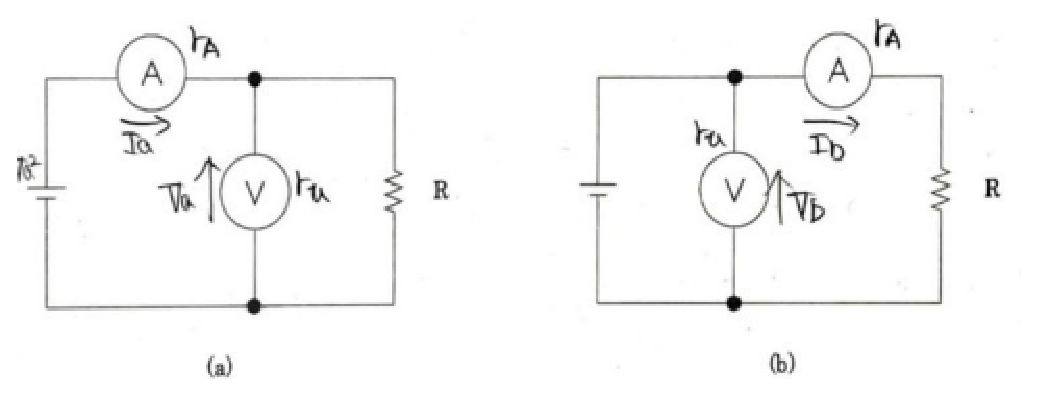
\includegraphics[width=15cm]{fig3.eps}
  \caption{}\label{fig1}
\end{figure}

\subsection{計器の内部抵抗を考慮した場合、回路~(a)と~(b)で測定値からRを求める式をそれぞれ示しなさい。}
図\ref{fig1}~(a)より、電圧源の電圧を$V$とすると、
\begin{align}
  V&=r_{A}I_{a}+V_{a}\label{eq1}\\
  V&=r_{A}I_{a}+R\left(I_{a}-\frac{V_{a}}{r_{v}}\right)\label{eq2}
\end{align}

式\eqref{eq1},~\eqref{eq2}より、

\begin{align}
  \begin{split}
  V_{a}
  &=R\left(I_{a}-\frac{V_{a}}{r_{v}}\right)\\
  R
  &=\frac{V_{a}}{\left(I_{a}-\frac{V_{a}}{r_{v}}\right)}\\
  &=\frac{r_{v}V_{a}}{r_{v}I_{a}-V_{a}}
  \end{split}\label{eq3}
\end{align}
となる。

また、図\ref{fig1}~(b)より、
\begin{align}
  \begin{split}
    V_{b}
    &=(r_{A}+R)I_{b}\\
    r_{A}+R
    &=\frac{V_{b}}{I_{b}}\\
    R
    &=\frac{V_{b}}{I_{b}}-r_{A}
  \end{split}\label{eq4}
\end{align}
となる。

\subsection{$\left|\Delta R/R\right|\leq 0.01$の精度で測定するためには、Rと内部抵抗の間にどのような関係があればよいか。回路~(a)と~(b)それぞれについて答えなさい。}

\paragraph{図\ref{fig1}~(a)}
測定値から求まる抵抗を$R_{m}$とすると、$R_{m}=\frac{V_{a}}{I_{a}}$であるから、測定誤差$\frac{\Delta R}{R}$は、式\eqref{eq3}より、
\begin{align}
  \begin{split}
    \frac{\Delta R}{R}
    &=\frac{R_{m}-R}{R}\\
    &=\frac{\frac{V_{a}}{I_{a}}-\frac{r_{v}V_{a}}{r_{v}I_{a}-V_{a}}}{\frac{r_{v}V_{a}}{r_{v}I_{a}-V_{a}}}\\
    &=\frac{\frac{V_{a}(r_{v}I_{a}-V_{a})}{I_{a}}-r_{v}V_{a}}{r_{v}V_{a}}\\
    &=\frac{\frac{V_{a}(r_{v}I_{a})}{I_{a}}-\frac{V_{a}^{2}}{I_{a}}-r_{v}V_{a}}{r_{v}V_{a}}\\
    &=-\frac{V_{a}}{r_{v}I_{a}}
    \label{eq5}
  \end{split}
\end{align}
となる。$I_{a}=\frac{V_{a}}{\frac{Rr_{v}}{R+r_{v}}}=\frac{V_{a}(R+r_{v})}{Rr_{v}}$より、
\begin{align}
  \begin{split}
    \frac{\Delta R}{R}
    &=-\frac{V_{a}}{r_{v}\frac{V_{a}(R+r_{v})}{Rr_{v}}}\\
    &=-\frac{R}{R+r_{v}}
    \label{eq6}
  \end{split}
\end{align}
となるから、
\begin{align}
  \begin{split}
    \left|\frac{\Delta R}{R}\right|=\left|-\frac{R}{R+r_{v}}\right|=\frac{R}{R+r_{v}}
    &\leq 0.01\\
    R
    &\leq 0.01(R+r_{v})\\
    0.99R
    &\leq 0.01r_{v}\\
    R
    &\leq \frac{1}{99}r_{v}
    \label{eq7}
  \end{split}
\end{align}
となる。

\paragraph{図\ref{fig1}~(b)}
測定値から求まる抵抗を$R_{m}$とすると、$R_{m}=\frac{V_{b}}{I_{b}}$であるから、測定誤差$\frac{\Delta R}{R}$は、式\eqref{eq4}より、
\begin{align}
  \begin{split}
    \frac{\Delta R}{R}
    &=\frac{R_{m}-R}{R}\\
    &=\frac{\frac{V_{b}}{I_{b}}-\left(\frac{V_{b}}{I_{b}}-r_{A}\right)}{R}\\
    &=\frac{r_{A}}{R}
    \label{eq8}
  \end{split}
\end{align}
となるから、
\begin{align}
  \begin{split}
    \left|\frac{\Delta R}{R}\right|=\left|\frac{r_{A}}{R}\right|=\frac{r_{A}}{R}
    &\leq 0.01\\
    R
    &\geq 100r_{A}
    \label{eq9}
  \end{split}
\end{align}
となる。

\subsection{内部抵抗を無視して測定値のみで$R$の値を求める場合、それぞれどのような$R$の範囲の測定に適しているか答えなさい。}
図\ref{fig1}~(a)では、$R\ll r_{v}$であるため、$R$の値が大きい測定に適しており、図\ref{fig1}~(b)では、$R\gg r_{v}$であるため、$R$の値が小さい測定に適している。

\end{document}